Minding meeting the requirements established in Chapter~\ref{sec:protocol-fundamentals}, the system design process and infrastructure choices for accomplishing the establishment of a Mesh Network were crucial in ensuring its operability. The following sections describe the design of the system and the testbed setup, as well as the challenges faced during the establishment of the network infrastructure.

\subsubsection{System Design} \label{sec:infrastructure}

One of the critical decisions was the selection of an appropriate operating system (OS) for configuring and enabling an ad hoc and dynamic Mesh Network. Multiple Linux distributions were initially explored, including OpenWrt, Raspbian, Ubuntu, and others. After careful consideration and a handful of failed attempts, OpenWrt led the track to host the protocol implementation. Its automated build tools and configurable packages, including the straightforward \emph{batman-adv} kernel module integration, load, and setup, made it a suitable choice for the high level flexibility and customization of the mesh network. The OS's active development community and extensive documentation further supported its use. As mentioned in Section~\ref{sec:background-wireless-mesh-networks}, OpenWrt is a lightweight solution for embedded devices, supporting a considerable set of platforms and toolchains for targetted integration of embedded software. Its choice turned out to be strategic regarding as well the role played in the spawning of decentralized and community-driven computer networks, that actively contribute to and are powered by such open source projects, all around the world\footnote{\url{https://en.wikipedia.org/w/index.php?title=Freifunk}}.

The OpenWrt image building process took advantage of the official Image Builder pre-compiled environment in order to create a custom image, skipping the need for source compilation\footnote{\url{https://openwrt.org/docs/guide-user/additional-software/imagebuilder}}. The image building process was automated with the help of a \emph{Dockerfile}, not only to allow for an easy integration and further testing of the mesh network related pre-compiled packages, but also to enable the experimentation with different network settings and the quick embedding and deployment of the \pol{} protocol software. The packages were chosen to provide deployment and debugging support for mesh networking using \emph{batman-adv}, wireless security using WPA/WPA2, working with the \emph{ext4} file system, and interacting with an Ethereum network via the official \emph{geth} client. The images were experimentally compiled for \emph{x86-64}, \emph{bcm2708}, and \emph{bcm2709} targets, being the last two ideal for the Raspberry Pi Zero and Raspberry Pi 2/3/4 models, respectively\footnote{\url{https://firmware-selector.openwrt.org/}}.

\subsubsection{Testbed Setup} \label{sec:infrastructure:testbed}

% Raspberry Pi failure deploymment
% Choice for QEMU for ease of testing and deployment
% Description of the testbed, including the hardware emulated, characteristics, etc.
% Description of the tap and bridge interfaces, etc.

The next step was to set up a testing environment for the deployment and running of the \pol{} protocol. Up to the delivery of this thesis, efforts are being made to port the generated OpenWrt image and compiled protocol modules to physical Raspberry Pis. However, the deployment on physical devices and the configuration of wireless interfaces is proving to be a challenge on multiple levels. The current drawbacks being faced are related to the automated enabling of the \emph{batman-adv} kernel module, in order to allow for the autonomous start of a dynamic and ad hoc mesh network. Nevertheless, even when manually configuring the interfaces, the protocol process of dynamic neighbourhood discovery is also failing, as the wireless interfaces are not able to easily detect each other, or establish a stable connection. Further investigations are being made to identify the root cause of these problems, and to finally uncover the solution for the deployment of the protocol on physical devices. These attempts and the physical demonstration of the \pol{} protocol are set for future work.

Meanwhile, to ease such development and testing hustle and to allow for a more flexible and faster deployment of the protocol, a virtualized environment was set up using QEMU (see Section~\ref{sec:background-wireless-mesh-networks}). The environment was configured to emulate a set of \emph{x86-64} target devices, and to run the OpenWrt image with the embedded and target-compiled \pol{} software. The testbed setup followed the guidelines of the official \emph{batman-adv} documentation\footnote{\url{https://www.open-mesh.org/doc/devtools/Emulation_Environment.html}}. To reduce manual input, an automated script was programmed, expecting the previously built OpenWrt image, and defining variables for the instance type, either “witness” or “prover”, the instance number, and a GDB port number, for kernel debugging. The script creates a shared bridge for the cluster and a unique tap interface for each virtual machine, assigning to them an individual MAC address. Finally, the script launches QEMU by creating a new virtual disk image, as a copy-on-write snapshot of the OpenWrt image, and by setting up each virtual machine with 1 GB of memory, 2 virtual CPUs, and a virtual SCSI disk. It assigns, as well, network interfaces to the instances. One uses the previously created tap interface to flush the mesh network traffic, and a second one is a virtual NIC to allow for the usual internet connection\footnote{\url{https://www.open-mesh.org/doc/devtools/OpenWrt_in_QEMU.html}}. KVM is also enabled in order to speed up the emulation, as well as a virtual RNG (Random Number Generator) and a virtual serial port. Up and running, with three witnesses and a prover instance, the testbed looks as depicted in Figure~\ref{fig:infrastructure:testbed}.

\begin{figure}[h!]
    \begin{center}
    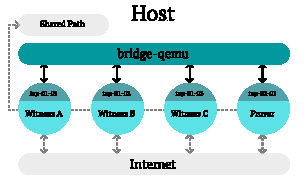
\includegraphics[width=0.9\textwidth]{proof-of-concept-qemu.pdf}
    \caption{Testbed setup for the \pol{} protocol.}
    \label{fig:infrastructure:testbed}
    \end{center}
\end{figure}

\subsubsection{Network Architecture} \label{sec:infrastructure:network-architecture}

After the establishment of the testbed, the physical networking layer is emulated by the bridge interface, which is set to pool all the mesh traffic that flows into and from the tap interfaces. The step that follows is the configuration of the \emph{batman-adv} kernel module, responsible for the dynamic and ad hoc mesh network creation. This step was automated at the OpenWrt image building process, with the inclusion of custom instructions in the image startup scripts. These instructions set the routing algorithm and add the virtual Ethernet interface eth0, corresponding to the tap interface created before, to the batman-adv interface bat0. The interval time between the broadcasting of neighbourhood discovery messages is set to 5 seconds, which determines how often a node should broadcast its presence in the network, and the bridge loop avoidance mechanism is activated, penalizing the routing of traffic through routes with more hops. This last step is important to avoid the creation of loops in the network and to ensure that the traffic is always routed through the shortest path, i.e., forcing the nodes to communicate directly with each other, within the testbed. Finally, the script disables the firewall to avoid any interference with batman-adv, and flushes the IP addresses of both the eth0 and bat0 interfaces.

Subnetting is then done via the assignment of an IP address to the bat0 interface. The IP address of each instance is generated based on the MAC address of the network interface eth0, establishing a non-conflicting address in the 192.168.0.x/24 subnet. After this step, the network is ready to use the TCP/IP stack, and the \pol{} protocol can be deployed, configured, and run. The final network topology is depicted in Figure~\ref{fig:infrastructure:network-architecture}.

\begin{figure}[h!]
    \begin{center}
    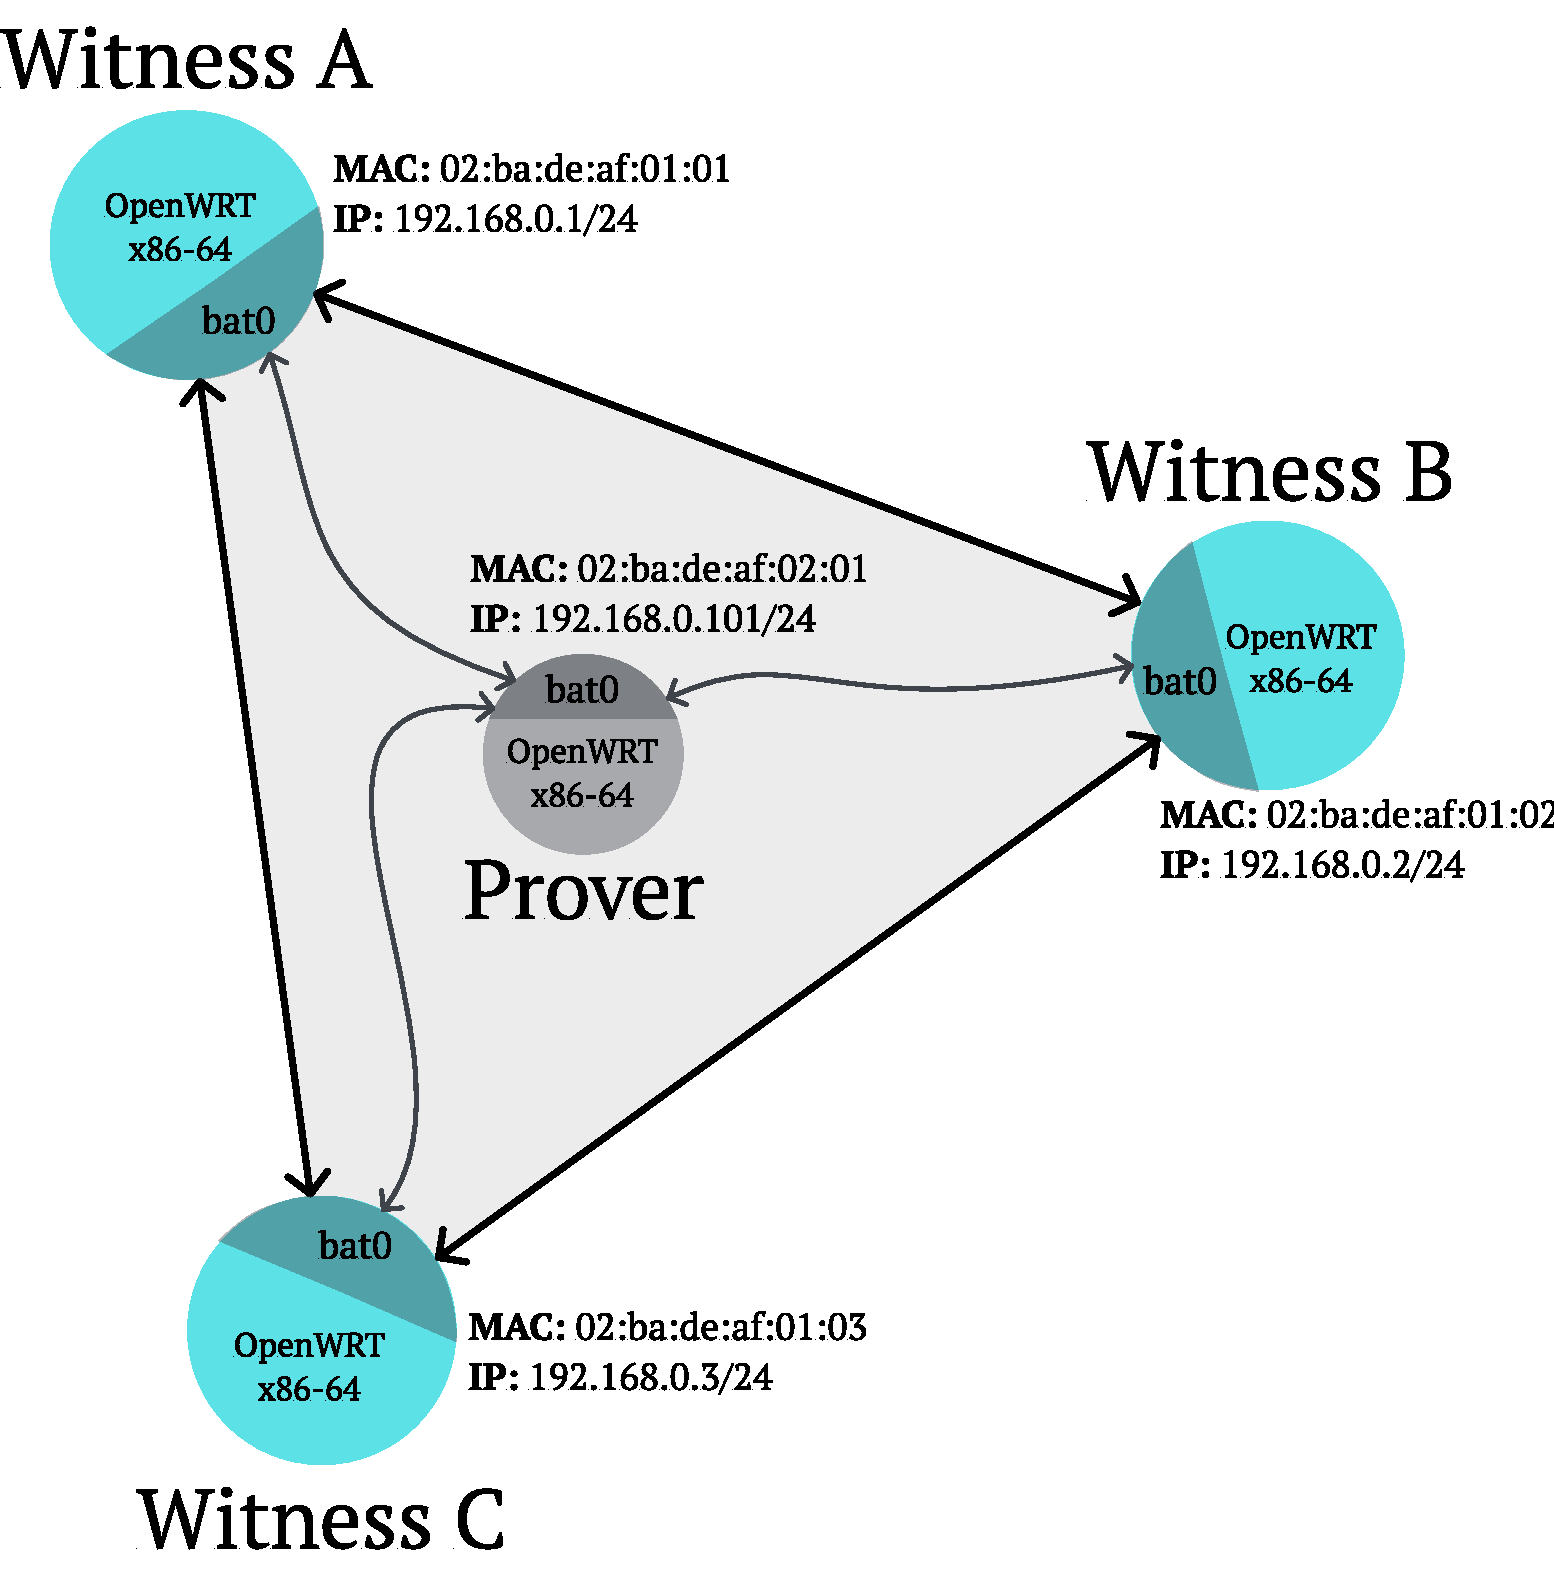
\includegraphics[width=0.7\textwidth]{proof-of-concept-network-topology.pdf}
    \caption{Network topology of the system under test, after configuring the \emph{batman-adv} interface and assigning IP addresses to the instances.}
    \label{fig:infrastructure:network-architecture}
    \end{center}
\end{figure}